\chapter{Overview}

\begin{figure}
    \begin{center}
    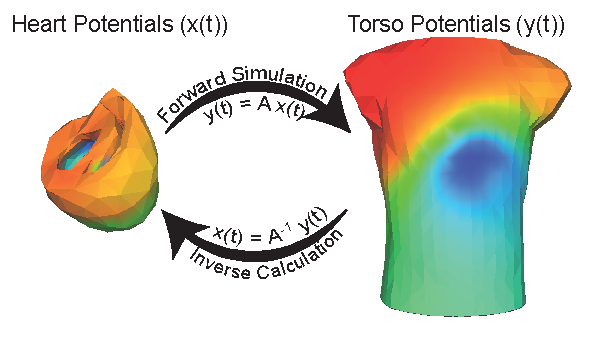
\includegraphics[width=0.75\textwidth]{ECGToolkitGuide_figures/fwd_inv_diag.pdf}
    \caption{Forward and inverse problems in electrocardiology.  The forward simulation involves 
        computing the torso potentials with know cardiac sources and torso geometry.  The inverse 
        solution, called ECG Imaging (ECG) consists of inverting the forward model to calculate cardiac
        sources from body surface recordings.}
    \label{fig:fwdinv_diag}
    \end{center}
    \end{figure}
    
\begin{introduction}

This guide describes and documents the SCIRun ECG Forward/Inverse
Toolkit. This toolkit is a collection of modules and networks
within the SCIRun system, which can be used to solve forward and inverse
electrocardiography problems. The guide assumes that the reader has basic
user-level familiarity with SCIRun; in particular that the reader is
familiar with placing modules into a SCIRun network, connecting modules,
and visualizing data. If the reader is not familiar with these operations,
we suggest you first consult the SCIRun Basic Tutorial, also distributed in
the SCIRun documentation.

The purpose of this toolkit is to advance the state of forward and inverse
solutions in this field by offering a common platform for investigators and
others to compare geometries and geometric representations, forward and 
inverse algorithms and data, with the maximum degree of both flexibility
and commonality that we can achieve. Thus, we hope to increase the
"reproducibility'' of developments in this field and help
move these technologies closer to useful clinical applications. As such, the
software (like all of SCIRun) is open-source, modular, and extensible. We
follow modern open-source software engineering practices to maximize
portability, extensibility, and reliability of our software. As we explain below, SCIRun has a
built-in facility for connecting with Python, or Matlab through Python, so that processing can be
carried out jointly using both programs. In
addition, the ECG Forward/Inverse Toolkit features capabilities which allow
the user to interface with ECGSim (\href{http://www.ecgsim.org}{http://www.ecgsim.org}), a
popular software package for solving certain types of forward ECG problems
with a high degree of interactive control over source models).

We welcome inquiries from users about this toolkit, and very much encourage
contributions to the toolkit from the community. For more information
about the toolkit or the underlying algorithms, or to discuss contributing to
its development, please contact \textit{scirun-users@sci.utah.edu}.

This toolkit is a product of the Center for Integrative Biomedical
Computing (CIBC), an NIH supported Biomedical Technology Research Center,
and we gratefully acknowledge the support from NIH that has made the
development of this work possible. The CIBC is housed in the Scientific
Computing and Imaging (SCI) Institute at the University of Utah and the
environment and personnel in SCI have also been integral to the development of the toolkit.

\end{introduction}

\section{Toolkit overview and capabilities}
    
Computational modeling of bioelectric fields often requires the solution of
electrocardiographic or electroencephalographic forward and inverse
problems in order to non-invasively analyze electrophysiological events
that are otherwise inaccessible or unethical to explore. All solutions to
both problems require a common set of components, each of which is then
customized or optimized for the particular problem formulation.
Bioelectric activity begins from a biophysical source of voltage or current,
which for computational purposes must be modeled in an appropriate,
problem-specific form. For example, when the clinical mission is to
identify focal activation in the brain, one or more current dipoles may be
a suitable source model. However, when the goal is to reconstruct the
sequence of activation across the ventricles of the heart, the sources are
better modeled in more complex form to capture the wavefront of this
activation. Each type of source then requires an approximation in
mathematical and then numerical form. Such a source model can then be used
(in a solution to the \textit{forward} problem) to computationally generate
the associated voltages on the surface of the body (or wherever
measurements might be made). If the goal is to recover sources from
measured potentials, \textit{i.e.} to solve the \textit{inverse} problem,
such as in the activation sequence reconstruction just mentioned, the
solution strategy must include appropriate numerical techniques that can
incorporate constraints and recover useful solutions, even when the inverse
problem is poorly posed and hence the forward problem numerically ill-conditioned.

Creating complete software solutions to such problems from scratch is a
daunting undertaking, requiring both considerable resources and considerable
breadth of expertise. It is in order to make such tools more accessible to
a broader array of researchers, and to enable validation and comparison
across solution approaches, that the Center for Integrative Biomedical
Computing (CIBC) has created this ECG Forward/Inverse toolkit. It is
designed to provide a generalized software environment, based on the open-source
SCIRun system, to aid researchers to construct, execute, visualize,
and compare such computational models.

SCIRun is based on a data flow-visual programming paradigm, in which distinct
computational (and software) modules are linked by connections (``data
pipes'') to form functional networks. The network editor offers the user
interactive control and flexibility to assemble the specific network needed to
solve the computational task at hand.
The ECG Forward/Inverse toolkit provides
a diverse array of modules, with associated data types, for bioelectric field problems,
together with sample networks and data sets with which to explore its
functionality.
An additional key feature of using the SCIRun system is
that rather than requiring custom code for all its functionality, the
toolkit leverages SCIRun's ability to
connect directly to Matlab through a
bi-directional Matlab interface, and has capabilities to read in data
created by ECGSim, as mentioned above.

Table \ref{tab:prop} lists currently available forward and inverse
approaches explicitly provided within the toolkit. The toolkit contains
full simulation example networks that illustrate potential and
activation-based forward models using both finite element (FEM) and boundary
element (BEM) approximation techniques as well as selected potential and
activation-based inverse methods. As indicated by the table,
simulation specific tools, such as lead field and stiffness matrix
generators, as well as a variety of regularization modules, are also
included, and can easily be included in user-built networks.

\begin{table}[htb]
\begin{tabular}{|ll|l|}
\hline
{\bf Forward tools} & {\bf Inverse Tools}\\ \hline
\hline
Potential-Based FEM/BEM$^\dag$ & Activation-Based$^{\&*\ddag}$\\ \hline
FEM Lead Field Calculation& Potential-Based Regularization  Methods\\ \hline
Stiffness Matrix Calculation &   -  Tikhonov  \\ \hline
 &- Tikhonov SVD  \\ \hline
 & - Truncated SVD\\ \hline
 & - Isotropy method$^{*}$\\ \hline
 & - Gauss-Newton Method$^{*\ddag}$\\ \hline
 & - Wavefront based potential reconstruction$^*$\\ \hline
 & - Total Variation$^{*}$ \\ \hline
 & - Method of Fundamental Solution (MFS) $^\ddag$\\ \hline
\end{tabular}
\caption{Algorithms currently included in the CIBC ECG Forward/Inverse
toolkit \newline
$^\dag$Activation-based forward solution is not yet
unavailable\newline
$^{\&}$Based on a Gauss-Newton optimization \newline
$^{*}$ Matlab implementation
$^\ddag$ Python implementation
}
\label{tab:prop}
\end{table}

\newpage

\section{Software requirements}

\subsection{SCIRun Compatibility}

The modules demonstrated in this tutorial are available in SCIRun
version 4.5 and higher. This tutorial is not compatible with earlier
 versions of SCIRun. If you have an existing SCIRun installation, we
 strongly encourage you to update your SCIRun version
to the latest build, available from the SCI software portal
(\href{http://software.sci.utah.edu}{http://software.sci.utah.edu}), which will include the latest bug
fixes and ensure that your version is up to date with the capabilities demonstrated in this guide.

\subsection{Required Datasets}

This tutorial relies on several datasets that are freely distributed as part of the
SCIRunData bundle. To obtain these datasets, please go to the SCI
software portal at \newline\href{http://software.sci.utah.edu}{http://software.sci.utah.edu} and click on {\bf
Download SCIRun} to download the SCIRunData zip files. The SCIRunData
dataset is provided in both zip and gzip file formats for your convenience.

